\documentclass[12pt]{article}

\usepackage{sbc-template}

\usepackage{graphicx,url}

\usepackage[brazil]{babel}   
%\usepackage[latin1]{inputenc}  
\usepackage[utf8]{inputenc}  
% UTF-8 encoding is recommended by ShareLaTex

% Para listar código font e comandos
\usepackage{minted}     

\sloppy

\title{Viabilidade do Uso Prático de Análise de Mutantes em Python}

\author{Sérgio Oliveira Campos\inst{1}, Ellen Francine Barbosa\inst{1}}

\address{Instituto de Ciências Matemáticas e Computação (ICMC) -- Universidade de São Paulo
  (USP)\\
  Avenida Trabalhador São-carlense, 400 - Centro -- 13566-590 -- São Carlos -- SP -- Brazil
  \email{seocam@usp.br, francine@icmc.usp.br}
}

\begin{document} 

\maketitle

\begin{abstract}
  This meta-paper describes the style to be used in articles and short papers
  for SBC conferences. For papers in English, you should add just an abstract
  while for the papers in Portuguese, we also ask for an abstract in
  Portuguese (``resumo''). In both cases, abstracts should not have more than
  10 lines and must be in the first page of the paper.
\end{abstract}
     
\begin{resumo} 
  Este meta-artigo descreve o estilo a ser usado na confecção de artigos e
  resumos de artigos para publicação nos anais das conferências organizadas
  pela SBC. É solicitada a escrita de resumo e abstract apenas para os artigos
  escritos em português. Artigos em inglês deverão apresentar apenas abstract.
  Nos dois casos, o autor deve tomar cuidado para que o resumo (e o abstract)
  não ultrapassem 10 linhas cada, sendo que ambos devem estar na primeira
  página do artigo.
\end{resumo}


\section{Introdução}


Análise de mutantes (ou teste de mutação) \cite{DeMillo:1978} é uma técnica 
utilizada para avaliar a qualidade de um conjunto de casos de teste. 
A técnica consiste
na alteração proposital de pequenos trechos de códigos afim de introduzir erros na
execução do programa. Apenas uma alteração é realizada por vez e os casos
de teste são executados novamente para cada uma das versões alteradas do
programa, denominadas mutantes.

Se ao menos um caso de teste fizer o programa
mutante se comportar de forma diferente do programa original, o mutante é dito 
``morto''. Quando um mutante tem comportamento comprovadamente idêntico ao 
programa original, o mutante não poderá ser morto e, neste caso, o mutante é
chamado de ``equivalente''. Cada alteração realizada no programa original é 
feita programaticamente através de
rotinas pré-determinadas. Estas rotinas, chamadas de operadores de mutação, variam
de acordo com cada linguagem.

Estudos realizados \cite{Frankl:1993, Li:2009, Andrews:2005} apontam que
o uso da análise de mutantes é mais efetiva do que outros critérios de 
cobertura em termos de detecção de falha; Devido ao alto custo da técnica
\cite{Gopinath:2014} chegou a conclusão que, na prática, o critério 
mais adequado para ser utilizado por desenvolvedores seria o de ``cobertura
de nós''. Em \cite{Li:2015}, relatam seus estudos sobre os desafios de se 
utilizar a análise de mutantes na prática com a linguagem Ruby, e chegam
a conclusão de que com adaptações na ferramenta testada (muRuby) a adoção
do critério seria viável.

Este artigo visa levantar quais são os fatores limitantes para o uso da análise
de mutantes durante o desenvolvimento de projetos Python reais.


\section{Análise de Mutantes em Python}

O Python é uma linguagem de programação de auto-nível, interpretada e de tipagem
dinâmica criada em 1991 por Guido Van Rossum e atualmente é mantida pela 
Python Software Foundation\footnotemark. Sua implementação de referência é o 
interpretador CPython escrito na linguagem C.

\footnotetext{Python Software Foundation -- https://www.python.org/}

Nessa seção será introduzido o estado atual da análise de mutantes na
linguagem Python.

\subsection{Mutantes Incompetentes}

Pelo fato de ser uma linguagem de tipagem dinâmica o interpretador Python não
é capaz de saber o tipo de uma determinada variável até o momento de sua
atribuição. Além disso o tipo de uma variável também pode ser alterado durante a 
execução do programa dentro de um mesmo escopo.

Por este motivo, o processo de criação de mutantes em Python estaria 
suscetível a gerar um maior número de mutantes com falhas consideradas
graves \cite{Bessam:2014}, que encerram a execução do programa antes do 
esperado, e por isso não são úteis na detecção de falhas no programa testado.
Este tipo de mutantes são chamados mutantes incompetentes \cite{Bottaci:2010}.

\subsection{Operadores de Mutação Suportados}

O potencial para geração de mutantes incompetentes é um problema para
a utilização de operadores de mutação propostos para outras linguagens,
além de limitar a criação de novos operadores. Hoje a linguagem Python conta com 20 operadores
de mutação, descritos por \cite{Derezinska:2014} e implementados na ferramenta
\textit{MutPy}\footnotemark, são estes:

\renewcommand{\labelitemi}{}
\begin{itemize}
    \item \textit{AOD} - arithmetic operator deletion
    \item \textit{AOR} - arithmetic operator replacement
    \item \textit{ASR} - assignment operator replacement
    \item \textit{BCR} - break continue replacement
    \item \textit{COD} - conditional operator deletion
    \item \textit{COI} - conditional operator insertion
    \item \textit{CRP} - constant replacement
    \item \textit{DDL} - decorator deletion
    \item \textit{EHD} - exception handler deletion
    \item \textit{EXS} - exception swallowing
    \item \textit{IHD} - hiding variable deletion
    \item \textit{IOD} - overriding method deletion
    \item \textit{IOP} - overridden method calling position change
    \item \textit{LCR} - logical connector replacement
    \item \textit{LOD} - logical operator deletion
    \item \textit{LOR} - logical operator replacement
    \item \textit{ROR} - relational operator replacement
    \item \textit{SCD} - super calling deletion
    \item \textit{SCI} - super calling insert
    \item \textit{SIR} - slice index remove
\end{itemize}


A linguagem C e a linguagem Ruby, por exemplo, contam com 71 \cite{Delamaro:1996} e 
54 operadores respectivamente \cite{Li:2015} (implementados nas 
ferramentas \textit{PROTEUM} e \textit{muRuby}).

\subsection{Ferramentas Python para Análise de Mutantes}


\footnotetext{MutPy -- https://bitbucket.org/khalas/mutpy}


\section{Trabalhos Relacionados}

\subsection{Aplicação Prática de Análise de Mutantes}

\section{Experimentos}

Para a verificação da viabilidade da utilização da análise
de mutantes em projetos Python optamos por utilizar a 
ferramenta MutPy por se tratar da única ferramenta com
desenvolvimento ativo, além de ser a mais completa até o
momento.

Todos os procedimentos descritos neste artigo foram realizados
em um laptop pessoal, 2.8 GHz Intel Core i7, 16 GB de memória
RAM 1600 MHz DDR3 e armazenamento do tipo SSD.

O interpretador Python utilizado para realizar os testes foi o
CPython versão 3.3.6.

\subsection{Seleção dos Projetos}

Para a realização dos testes foram escolhidos quatro softwares
amplamente utilizados entre desenvolvedores os desenvolvedores
Python. Para a escolha a busca do portal Github\footnotemark 
foi utilizada para filtrar projetos da linguagem Python 
com pelo menos 1000 \textit{ forks}, 1000 estrelas e 1000 
seguidores. A string the busca utilizada foi:

\footnotetext{Github - https://github.com}

\begin{minted}{bash}
language:Python stars:>1000 forks:>1000 followers:>1000
\end{minted}

Além dos 4 primeiros projetos foi incluído um quinto projeto
cujo um dos autores deste artigo também é autor. O objetivo 
desta inserção foi de utilizar o projeto como \textit{benchmark}
da qualidade dos resultados apresentados pela ferramenta
MutPy, uma vez que parar analisar a equivalência de mutantes
é importante que o desenvolvedor tenha amplo conhecimento do
código.

Cada uma das ferramentas tiveram seu conjunto de casos de
testes executado conforme indicado por sua respectivas
documentações. Para a execução do testes foi utilizada a
\textit{branch} \textbf{master} de cada repositório.

Após a execução dos testes um dos projetos foi excluído da
lista inicial pois 21 dos 185 testes geravam erros durante a 
execução. 

A tabela \ref{tab:subjects} lista a seleção final de programas,
quantidade de linha código, quantidade de casos de teste e
tempo para execução de seus casos de teste.

\begin{table}[ht]
\centering
\caption{Projetos Python Analisados}
\label{tab:subjects}
\smallskip
\begin{tabular}{|l|c|c|c|}
\hline
Nome do Projeto & LOC (Python) & Casos de Teste & Tempo de execução dos testes\\[0.5ex]
\hline
&&&\\[-2ex]
Django & 581.108 & 10305 & 117.315s\\[0.5ex]
\hline
&&&\\[-2ex]
Flask & 13.894 & 257 & 2.071s\\[0.5ex]
\hline
&&&\\[-2ex]
Requests & 12.566 & 150 & 48.303s\\[0.5ex]
\hline
&&&\\[-2ex]
django-revproxy & 1.527 & 81 & 2.050s\\[0.5ex]
\hline
\end{tabular}
\end{table}

\subsection{Execução da MutPy}

Nesta seção são apresentados os procedimentos realizados para
a execução da MutPy para cada uma das ferramentas selecionadas.
Também serão apresentadas as dificuldades encontradas em cada
caso. Os relatórios gerados pela MutPy estarão disponíveis
para download e não serão anexados ao artigo devido a grande
quantidade de dados.

\subsubsection{Django}

Para executar a geração de mutantes no \textbf{Django} o comando
a seguir foi utilizado:

\begin{minted}{bash}
mut.py --target django --unit-test tests \
       --report-html report/
\end{minted}

A execução inicial da MutPy não conseguiu realizar a execução de
nenhum teste e também falhou ao tentar realizar a geração de
mutantes.

\subsubsection{Flask}

O comando utilizado para executar os MutPy com o \textbf{Flask} foi:

\begin{minted}{bash}
mut.py --target flask --unit-test tests \
       --report-html report/
\end{minted}

Para o \textbf{Flask} execução da inicial da MutPy falhou. 
A MutPy realiza uma busca por testes
dentro de pacotes e módulos Python porém não é capaz de encontrar
casos de testes dentro de diretórios. Para corrigir este problema 
o diretório de teste foi modificado para um módulo Python.

Após a intervenção foi realizada uma nova tentativa, desta vez a
ferramenta foi capaz de gerar 1871 mutantes porém novamente, nenhum 
caso de  teste foi encontrado, e por isso, nenhum mutante foi morto.

\subsubsection{Requests}

Ao realizar a execução dos testes para o programa \textbf{requests} foi
utilizado o comando:

\begin{minted}{bash}
mut.py --target requests --unit-test test_requests \
       --report-html report/
\end{minted}

Nessa tentativa a MutPy conseguiu realizar a execução inicial dos casos 
de teste porém ao tentar iniciar a geração dos mutantes ela encerrou gerando 
um erro do tipo \textit{ImportError}. 
Após analisar a causa da falha foi possível
detectar que a ferramenta abre cada módulo do programa e importa
para tentar realizar a mutação mesmo que este módulo não seja utilizado.
No caso do \textbf{requests} existem módulos que tem sua utilização
determinada de acordo com a versão do interpretador Python utilizado, para 
assim, manter a compatibilidade entre diferentes versões.

Além disso o \textbf{requests} distribui suas dependências junto com o
seu código e por não ser capaz de realizar tal diferenciação a geração 
de mutantes ocorre tanto para o código-fonte real como as dependências.

Para tentar mitigar o problema os arquivos de outras versões foram
excluídos e a MutPy foi executada novamente. Na nova execução os testes
foram executados, a geração de mutantes foi iniciada, porém
após a criação de 130 mutantes a MutPy encerrou com erro pois não foi
capaz de processar a constante \textit{\_\_file\_\_}.

Para dar continuidade ao processo de geração de mutantes as 
ocorrências da constante foram substituída pelas strings que deveriam ter
sido resolvida pelo interpretador (tanto no fonte como nas dependências).
Após a intervenção a execução foi novamente realizada.

Na nova execução 310 mutantes foram gerados até que a execução foi
interrompida pois houve falha na importação do módulo \textit{os}, nativo
da linguagem Python, 

Após essa última falha as tentativas de realizar os testes com o projeto
\textbf{requests} foram encerradas.

\subsubsection{django-revproxy}

Para realizar os testes do \textbf{django-revproxy} o comando a seguir
foi utilizado:

\begin{minted}{bash}
mut.py --target revproxy --unit-test tests \
       --report-html report/
\end{minted}

Na tentativa inicial de realizar os testes a MutPy encerrou pois
um dos testes unitários falhou. Os testes foram novamente executados,
sem a utilização da MutPy e foi constatado que não haviam problemas no
conjunto de testes porém, para dar continuidade aos testes o teste 
conflitante foi comentado. 

Após a intervenção os testes foram executados normalmente pela MutPy
e o processo de geração de mutantes e análise de mutantes foi concluído
com sucesso.

\section{Discussão}

PORQUE O PATCH FOI PRECISO

TEMPO DE EXECUÇÃO

NÃO É POSSÍVEL MARCAR MUTANTES EQUIVALENTES

FUNCIONA APENAS COM PYTHON 3

IMPORTA TODOS OS ARQUIVOS SENDO UTILIZADOS OU NÃO. DEVERIA SER POSSIVEL SELECIONAR ARQUIVOS/DIRETORIOS
PARA SEREM EXCLUIDOS

OUTRO PROBLEMA AO EXECUTAR A ANALISE NA REQUESTS EH QUE ELA MANTEM AS SUAS DEPENDENCIAS DENTRO DO PROPRIO REPOSITORIO
ASSIM COMO O DJANGO

RELATORIOS HTML DEVERIAM EXIBIR CODIGO LADO A LADO

OUTROS TIPOS DE MUTANTES

QUANDO UM TESTE FALHA NA ETAPA INICIAL NENHUM FEEDBACK SOBRE O QUE FALHOU E DADO

TEM PROBLEMAS PARA LIDAR COM CAMINHOS TANTO PARA IMPORTS COMO PARA FILES

A FORMA COMO OS IMPORTS SAO FEITOS AFETA A INTERPRETACAO DE CONSTANTES "MAGICAS" DA LINGUAGEM, COMO O \_\_FILE\_\_



\section{Resultados}

TABELA

PROBLEMAS EM MUTANTES ENCONTRADOS (FALSOS TIMEOUTS e INCOMPETENTES)

PROBLEMAS DE CONFLITOS COM O MOCK

VELOCIDADE DA COBERTURA

\section{Ameaças a validade}

O PATCH APLICADO PODE TER AFETADO O FUNCIONAMENTO.

AS ALTERAÇÕES NECESSARIAS EM CADA FERRAMENTA PODEM TER INFLUENCIADO OS RESULTADOS

\section{Conclusões}

AS FERRAMENTAS PYTHON AINDA NÃO ESTÃO PRONTAS PARA USO EM AMBIENTES REAIS








\section{Figures and Captions}\label{sec:figs}


Figure and table captions should be centered if less than one line
(Figure~\ref{fig:exampleFig1}), otherwise justified and indented by 0.8cm on
both margins, as shown in Figure~\ref{fig:exampleFig2}. The caption font must
be Helvetica, 10 point, boldface, with 6 points of space before and after each
caption.

\begin{figure}[ht]
\centering
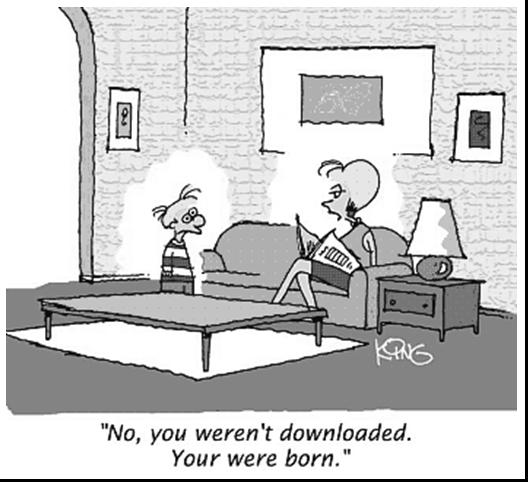
\includegraphics[width=.5\textwidth]{fig1.jpg}
\caption{A typical figure}
\label{fig:exampleFig1}
\end{figure}

\begin{figure}[ht]
\centering
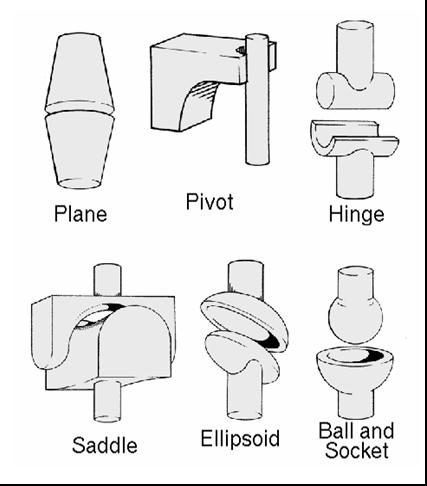
\includegraphics[width=.3\textwidth]{fig2.jpg}
\caption{This figure is an example of a figure caption taking more than one
  line and justified considering margins mentioned in Section~\ref{sec:figs}.}
\label{fig:exampleFig2}
\end{figure}

In tables, try to avoid the use of colored or shaded backgrounds, and avoid
thick, doubled, or unnecessary framing lines. When reporting empirical data,
do not use more decimal digits than warranted by their precision and
reproducibility. Table caption must be placed before the table (see Table 1)
and the font used must also be Helvetica, 10 point, boldface, with 6 points of
space before and after each caption.

\begin{table}[ht]
\centering
\caption{Variables to be considered on the evaluation of interaction
  techniques}
\label{tab:exTable1}
\smallskip
\begin{tabular}{|l|c|c|}
\hline
& Value 1 & Value 2\\[0.5ex]
\hline
&&\\[-2ex]
Case 1 & 1.0 $\pm$ 0.1 & 1.75$\times$10$^{-5}$ $\pm$ 5$\times$10$^{-7}$\\[0.5ex]
\hline
&&\\[-2ex]
Case 2 & 0.003(1) & 100.0\\[0.5ex]
\hline
\end{tabular}
\end{table}

\section{Images}

All images and illustrations should be in black-and-white, or gray tones,
excepting for the papers that will be electronically available (on CD-ROMs,
internet, etc.). The image resolution on paper should be about 600 dpi for
black-and-white images, and 150-300 dpi for grayscale images.  Do not include
images with excessive resolution, as they may take hours to print, without any
visible difference in the result. 


\bibliographystyle{sbc}
\bibliography{sbc-template}

\end{document}
